\documentclass{article}
\usepackage{graphicx}

\begin{document}
\newcommand{\todo}[1]{\vspace{0.5cm} \large \textbf{\underline{TODO}}\\ \normalsize #1 \vspace{0.5cm}}
\title{Documentation to the Online Exercise Assistant}
\author{Sylvia Stuurman}
\date{july 2008}
\maketitle
\begin{figure}[h]
\begin{center}
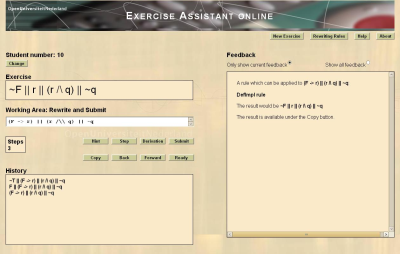
\includegraphics{figures/page-elements.png}
\end{center}
\caption{The Exercise Assistant On-line}\label{figure:screenshot}
\end{figure}
Below, we describe the static and dynamic structure of the code of the Exercise Assistant which uses the strategy-based feedback services.

\section{The HTML}
\subsection{The generic part}
The generic part of HTML for the Exercise Assistant is bundled in one file, which contains several elements which can be questioned and modified dynamically using Javascript, as we will see below. This file is written in PHP, and uses
php functions to write the labels in the page, to enable multilanguage usage (we will discuss where and how below)). The exact code is shown in appendix~\ref{appendix:framework}. 

The page elements (see figure~\ref{figure:screenshot}) are:
\begin{itemize}
\item a row of menubuttons immediately below the header, containing:
	\begin{itemize}
	\item The \textbf{New Exercise} button, which will invoke a \textbf{generate} function,
	\item The \textbf{Rules}-, \textbf{Help}- and \textbf{About}-buttons, which will cause three different HTML fragment to show,
		\end{itemize}
\item a left column, containing:
	\begin{itemize}
	\item In the OU version, page elements for input and display of the \textbf{student number}.
	\item The \textbf{Exercise Area} where the exercise will be shown (not editable by the user),
	\item The \textbf{Work Area} where the user may rewrite the expression,
	\item The \textbf{Progress Area} which will show how many steps will be needed minimally,
	\item two rows of buttons:
		\begin{itemize}
		\item The \textbf{Hint}-button which will invoke the hint function,
		\item The \textbf{Next}-button which will invoke the next function,
		\item The \textbf{Derivation}-button which will invoke the derivation function,
		\item The \textbf{Submit}-button which will invoke the feedback function,
		\item The \textbf{Copy}-button (only visible when there is something to copy) which will invoke the copy function,
		\item The \textbf{Back}-button (only visible when there is something to go back to) which will invoke the back function,
		\item The \textbf{Forward}-button (only visible when there is something to go forward to) which will invoke the forward function,
		\item The \textbf{Ready}-button which will invoke the ready function,
		\item In the domain-specific version, a virtual keyboard
		\end{itemize}
	\item The \textbf{History Area} which will show the valid steps,
	\end{itemize}
\item a right column, containing:
	\begin{itemize}
	\item two radiobuttons enabling the user to choose between viewing all feedback or (default) only the
	current feedback
	\item a button to clear the feedback area
	\item The \textbf{Feedback Area} whic will show the feedback. There are radio buttons with which the user nmay choose between seeing all feedback, or only the current feedback,
		\end{itemize}

\end{itemize}

In the head, framework.php shows the following line:
\begin{verbatim}
<script type="text/javascript">
    var exercisekind = 
        <?php $kind = getKind(); echo "\"$kind\";"; ?>; 
    var id=421;
</script>
\end{verbatim}
The values that will be used for the Javascript variables exercisekind and id are set here. The value for 
exercisekind is received from a php-function getKind(). We will discuss later how and where we implement this function.

\section{How to invoke the Exercise Assistant}
At this moment, there are three different ways to use the on-line Exercise Assistant: 
\begin{itemize}
\item in a \textbf{generic} way, which automatically supports every domain and every exercisekind 
which is supported by the feedback services, 
\item in a way which makes it possible to add \textbf{domain-specific} page elements and page behaviour, 
such as the use of the official symbolss for a domain and a virtual keyboard for input,
\item for OU students, where the student is asked to enter his or her \textbf{studentnumber}.
\end{itemize}

\subsection{Generic}
\textbf{http://ideas.cs.uu.nl/genexas/} 

This URL shows links to the types of exercises that are
offered by the Strategy-based feedbackservices. The links are hard-coded, but when an
extra service would send a list of types of exercises, this service could be used to 
generate the list of links automatically.

\todo{Create a service which returns a list of exercisekinds, and use that service from this URL}

The links link to:

\textbf{generic.php?exercisekind=Proposition to DNF} and

\textbf{generic.php?exercisekind=Relational Algebra}.


The file ``generic.php'' (see appendix~\ref{{appendix:generic}}) inludes standard help-, about- and rules files, includes a file which sets the language into English, and includes the file ``common/generic.php''(see appendix~\ref{{appendix:common:generic}}).

This file contains the HTML which produces a page with the Exercise Assistant. The variable exercisekind in the url is used to set the value of a Javascript variable called exercisekind, which will be used for the calls to the feedback services.

\subsubsection{Language}
The language now is default set to English, but using the language options of the Apache server, it would be easy to switch to multilanguage. In that case, instead of a single index.php, there would be an index.en.php and an index.nl.php (etc), and instead of including the file with English names, the appropriate language file would be included.

The file structure is:\\
/genexas/index.php \\
/genexas/generic.php \\
/genexas/common/en.php \\
/genexas/common/nl.php \\
/genexas/common/generic.php \\
/genexas/common/en/about.php \\
/genexas/common/en/help.php \\

Changing to multilanguage would result in\\
/genexas/index.en.php \\
/genexas/index.nl.php \\
/genexas/generic.php (to be called with a language variable)\\
/genexas/common/en.php \\
/genexas/common/nl.php \\
/genexas/common/generic.php \\
/genexas/common/en/about.php \\
/genexas/common/en/help.php \\
/genexas/common/nl/about.php \\
/genexas/common/nl/help.php \\

\subsection{Specific}
Another way to use the Exercise Assistant is through two specific URL's: 

\textbf{http://ideas.cs.uu.nl/genexas/logic/todnf/index.php} \\ (which makes use of the multilanguage facility; because only English is fully implemented, it is safest to use http://ideas.cs.uu.nl/genexas/logic/todnf/index.en) or 

\textbf{http://ideas.cs.uu.nl/genexas/math/relationalgebra/index.php} \\ (for which the same applies, so preferrably use http://ideas.cs.uu.nl/genexas/math/relationalgebra/index.en).

The difference with the so-called generic url is, that it is possible to integrate domain-specific HTML and Javascript, for instance to enhance the user interface by providing real mathematical symbols instead of ASCII characters for input and output.

\section{OU specific}
At last, there is the possibility to use the Exercise Assistant for OU students, asking them for their student number:

\textbf{http://ideas.cs.uu.nl/genexas/logic/todnf/ou/}

In this case, the student number will be sent with each call to the strategy-based feedback services.

\section{Javascript}
\subsection{/genexas/common/javascript/services.js}
This file contains functions to call the strategy-services. Each function requires the input which is needed to call the service, and a callback function. The services are called through an asynchronous Ajax call, and the callback function will be called when the result has arrived.

The functions are:
\begin{itemize}
\item function ss\_generate(number, callback) 
\item function ss\_getReady(state, callback) 
\item function ss\_getHint(location, state, callback) 
\item function ss\_getNext(state, callback)
\item function ss\_getDerivation(state, callback)
\item function ss\_getRemaining(state, callback) 
\item function ss\_getFeedback(state, newexpression, callback)
\end{itemize}

\subsection{/genexas/common/javascript/communication.js}
The functions in this file function as a mediator between the elements of the HTML page and the services.js-functions. 

For each action that the user interface allows to, there are a pair of functions: one that knows where to get the appropriate paramteres from, and one that knows how to display the results. The display function is used as the callback function when calling a function from services.js.

The pairs of functions are:

\begin{itemize}
\item function generate() and function displayExercise(state)
\item function getHint() and function displayHint(listOfRules)
\item function getNext() and  function displayNext(rule, location, state) 
\end{itemize}

\appendix
\section{HTML code for the Exercise Assistant}
\subsection{/genexas/common/framework.php}\label{appendix:framework}
\subsubsection{The HEAD}
\begin{verbatim}
<!DOCTYPE HTML PUBLIC "-//W3C//DTD HTML 4.01//EN"
    "http://www.w3.org/TR/html4/strict.dtd">
<html>
<head>
<meta http-equiv="Content-Type" 
    content="text/html;charset=utf-8" >

<title>OU Exercise Assistant On-line</title>
<link rel="stylesheet" type="text/css" 
    href="/genexas/css/exas.css" >
<link rel="shortcut icon" type="image/x-icon" 
    href="/genexas/css/favicon.ico" >
<script type="text/javascript" 
    src="/genexas/common/javascript/prototype-1.6.0.2.js">
    </script> 
<script type="text/javascript" 
    src="/genexas/common/javascript/help.js">
    </script>
<script type="text/javascript" 
    src="/genexas/common/javascript/services.js">
    </script>
<script type="text/javascript" 
    src="/genexas/common/javascript/communication.js">
    </script>
<script type="text/javascript" 
    src="<?php print Local;?>">
    </script>
<script type="text/javascript">
    var exercisekind = 
        <?php $kind = getKind(); echo "\"$kind\";"; ?>; 
    var id=421;
</script>
<script type="text/javascript" 
    src="/genexas/common/javascript/init.js">
    </script>
</head>
\end{verbatim}
\subsubsection{The BODY}
\subsubsubsection{The header and menubuttons}
\begin{verbatim}
<h1>Exercise Assistant online</h1>
<div id="exasdiv">
<input class="menu" type="button" 
    id="aboutButton" value="<?php print About;?>" >
<input class="menu" type="button" 
    id="helpButton" value="<?php print Help;?>" >
<input class="menu" type="button" 
    id="rulesButton" value="<?php print Rules;?>" >
<input class="menu" type="button" 
    id="generateButton" value="<?php print NewExercise;?>" >
<br class="clear" >
\end{verbatim}
\subsubsubsection{The left column}
\begin{verbatim}
<div class="column left">

  <div id="numberinput" style="display: none">
    <h3>Please first fill in your student number</h3>
    <textarea id="number" rows="1" cols="12"></textarea>
    <input type="button" id="numberbutton" value="Enter">
  </div><!-- end div numberinput -->
	
  <div id="numberdisplay"  style="display: none">
    <h3 id="studentnumber"></h3>
    <input type="button" id="changenumberbutton" 
    value="Change">
  </div><!-- end div numberdisplay -->
	
  <h3><?php print Exercise;?></h3>
  <div id="exercise" >
  </div><!-- end div exercise -->

  <h3><?php print WorkArea;?></h3>

	<textarea id="work" rows="2" cols="40" >	
	</textarea><!-- end work area -->
	
  <!-- the buttons -->
  <input class="minibutton" 
    id="submitbutton" type="button" 
    value="<?php print Submit;?>" >	
  <input class="minibutton" 
    id="derivationbutton"  type="button" 
    value="<?php print Derivation;?>" >
  <input class="minibutton" 
    id="nextbutton"  type="button" 
    value="<?php print Step;?>" >
  <input class="minibutton" 
    id="hintbutton" type="button" 
    value="<?php print Hint;?>" >
  <div id="progress">Steps<br>0
  </div><!-- end div progress -->
	
  <br class="clear">
  <input class="minibutton" type="button" 
    id="readybutton" value="<?php print Ready;?>" >
  <input class="minibutton" type="button" 
    id="forwardbutton" value="<?php print Forward;?>" >
  <input class="minibutton" type="button" 
    id="undobutton" value="<?php print Back;?>" >
  <input class="minibutton" type="button" 
    id="copybutton" value="<?php print Copy;?>" >
  <!-- end buttons -->
  <br>
	
  <h3><?php print History;?></h3>
  <div id="history">
  </div><!-- end div history -->

</div><!-- end div column left -->
\end{verbatim}
\subsubsubsection{The right column}
\begin{verbatim}
<div class="column right">

  <h3><?php print Feedback ?></h3>
  <label class="feedbacklabel"><?php print ChooseClear;?>
    <input type="radio" name="feedbackchoice" 
      id="feedbackclearchoice" 
      checked value="chooseclear" >
  </label>
  <label class="feedbacklabel"><?php print ChooseKeep;?>
    <input type="radio" name="feedbackchoice"  
      id="feedbackeepchoice" 
      value="choosekeep" >
  </label>
  <input type="button" 
    id="clearbutton" 
    value="<?php print Clear;?>"  style="display: none">
		
  <div id="feedback" class="clear"><?php print Welcome;?>
  </div><!-- end div feedback -->

</div><!-- end div column right -->
\end{verbatim}
\subsubsubsection{The Help areas}
\begin{verbatim}
<div id="rules" class="helparea invisible">
  <input class="helpbutton" 
    id="closerulesButton" type="button" 
    value="<?php print Close;?>" >
    <?php rules();?>
</div><!-- end div rules -->

<div id="help" class="helparea invisible">
  <input class="helpbutton"  
    id="closehelpButton" type="button" 
    value="<?php print Close;?>" >
    <?php help();?>
</div><!-- end div help -->

<div id="about" class="helparea invisible">
  <input class="helpbutton"  
    id="closeaboutButton" type="button" 
    value="<?php print Close;?>" >
    <?php about();?>
</div><!-- end div about -->

</div><!-- end div exas -->
</body>
</html>
\end{verbatim}
\subsection{/genexas/generic.php}\label{appendix:generic}
\begin{verbatim}
<?php
function getKind() {
  return $_GET["exercisekind"];
}
function rules() {
  include_once("common/en/rules.html");
}
function help() {
  include_once("common/en/help.html");
}
function about() {
  include_once("common/en/about.html");
}
include_once("common/en.php");

include("common/framework.php");
?>
\end{verbatim}
\end{document}